\section{EQUIPMENT}

\subsection{Diagram of experimental apparatus}
\begin{figure}[H]
    \centering
    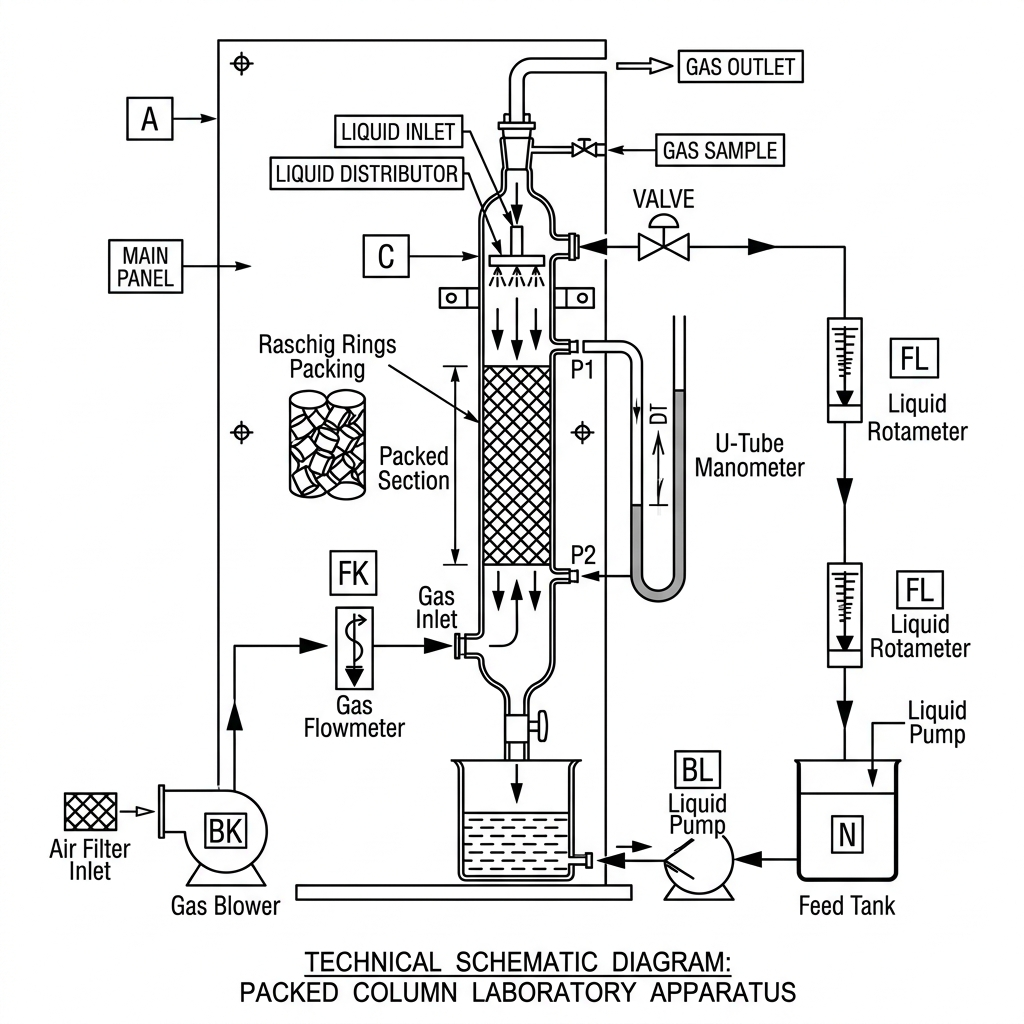
\includegraphics[width=0.8\textwidth]{Images/apparatus_diagram.png}
    \caption{Diagram of experimental apparatus}
\end{figure}
The experimental unit consists of:
\begin{enumerate}
    \item A glass column where Raschig rings are packed randomly.
    \item Gas feeding equipment: Air blower ($B_K$), gas pipe, U-tube manometer, differential pressure gauge, and gas flowmeter (scale 8-100\%, $V = 0.286$ $m^3$/min).
    \item Water feeding equipment: Feed tank ($N$), water pump ($B_L$), and liquid flowmeter (range 0-1.6, $G_L = 5.805$ l/min).
\end{enumerate}

\subsection{Characteristics of packed column}
\textbf{Glass column:}
\begin{itemize}
    \item Diameter: $d = 0.09$ m
    \item Height: $H = 0.805$ m
    \item Packing height: $Z = 0.42$ m
\end{itemize}

\textbf{Packing material (Raschig rings):}
\begin{itemize}
    \item Nominal diameter: $d = 12.7$ mm
    \item Specific surface area: $a = 370 - 380$ $m^2/m^3$
    \item Porosity: $\varepsilon = 0.586$
\end{itemize}

\subsection{List of components}
\begin{itemize}
    \item \textbf{A}: Panel
    \item \textbf{C}: Packed column
    \item \textbf{E}: Bottom part of column
    \item \textbf{$F_K$}: Gas flowmeter
    \item \textbf{g}: Liquid level device (pipe) at the bottom
    \item \textbf{$F_L$}: Liquid flowmeter
    \item \textbf{$B_K$}: Air blower (1.0 Hp)
    \item \textbf{$B_L$}: Liquid pump (0.5 Hp)
    \item \textbf{N}: Liquid tank
    \item \textbf{AK}: Pressure gauge
\end{itemize}
